\providecommand{\main}{../../../..}
\documentclass[\main/dresen_thesis.tex]{subfiles}
\begin{document}
  \label{sec:looselyPackedNS:nanoparticle:vsm}
  \begin{figure}[tb]
    \centering
    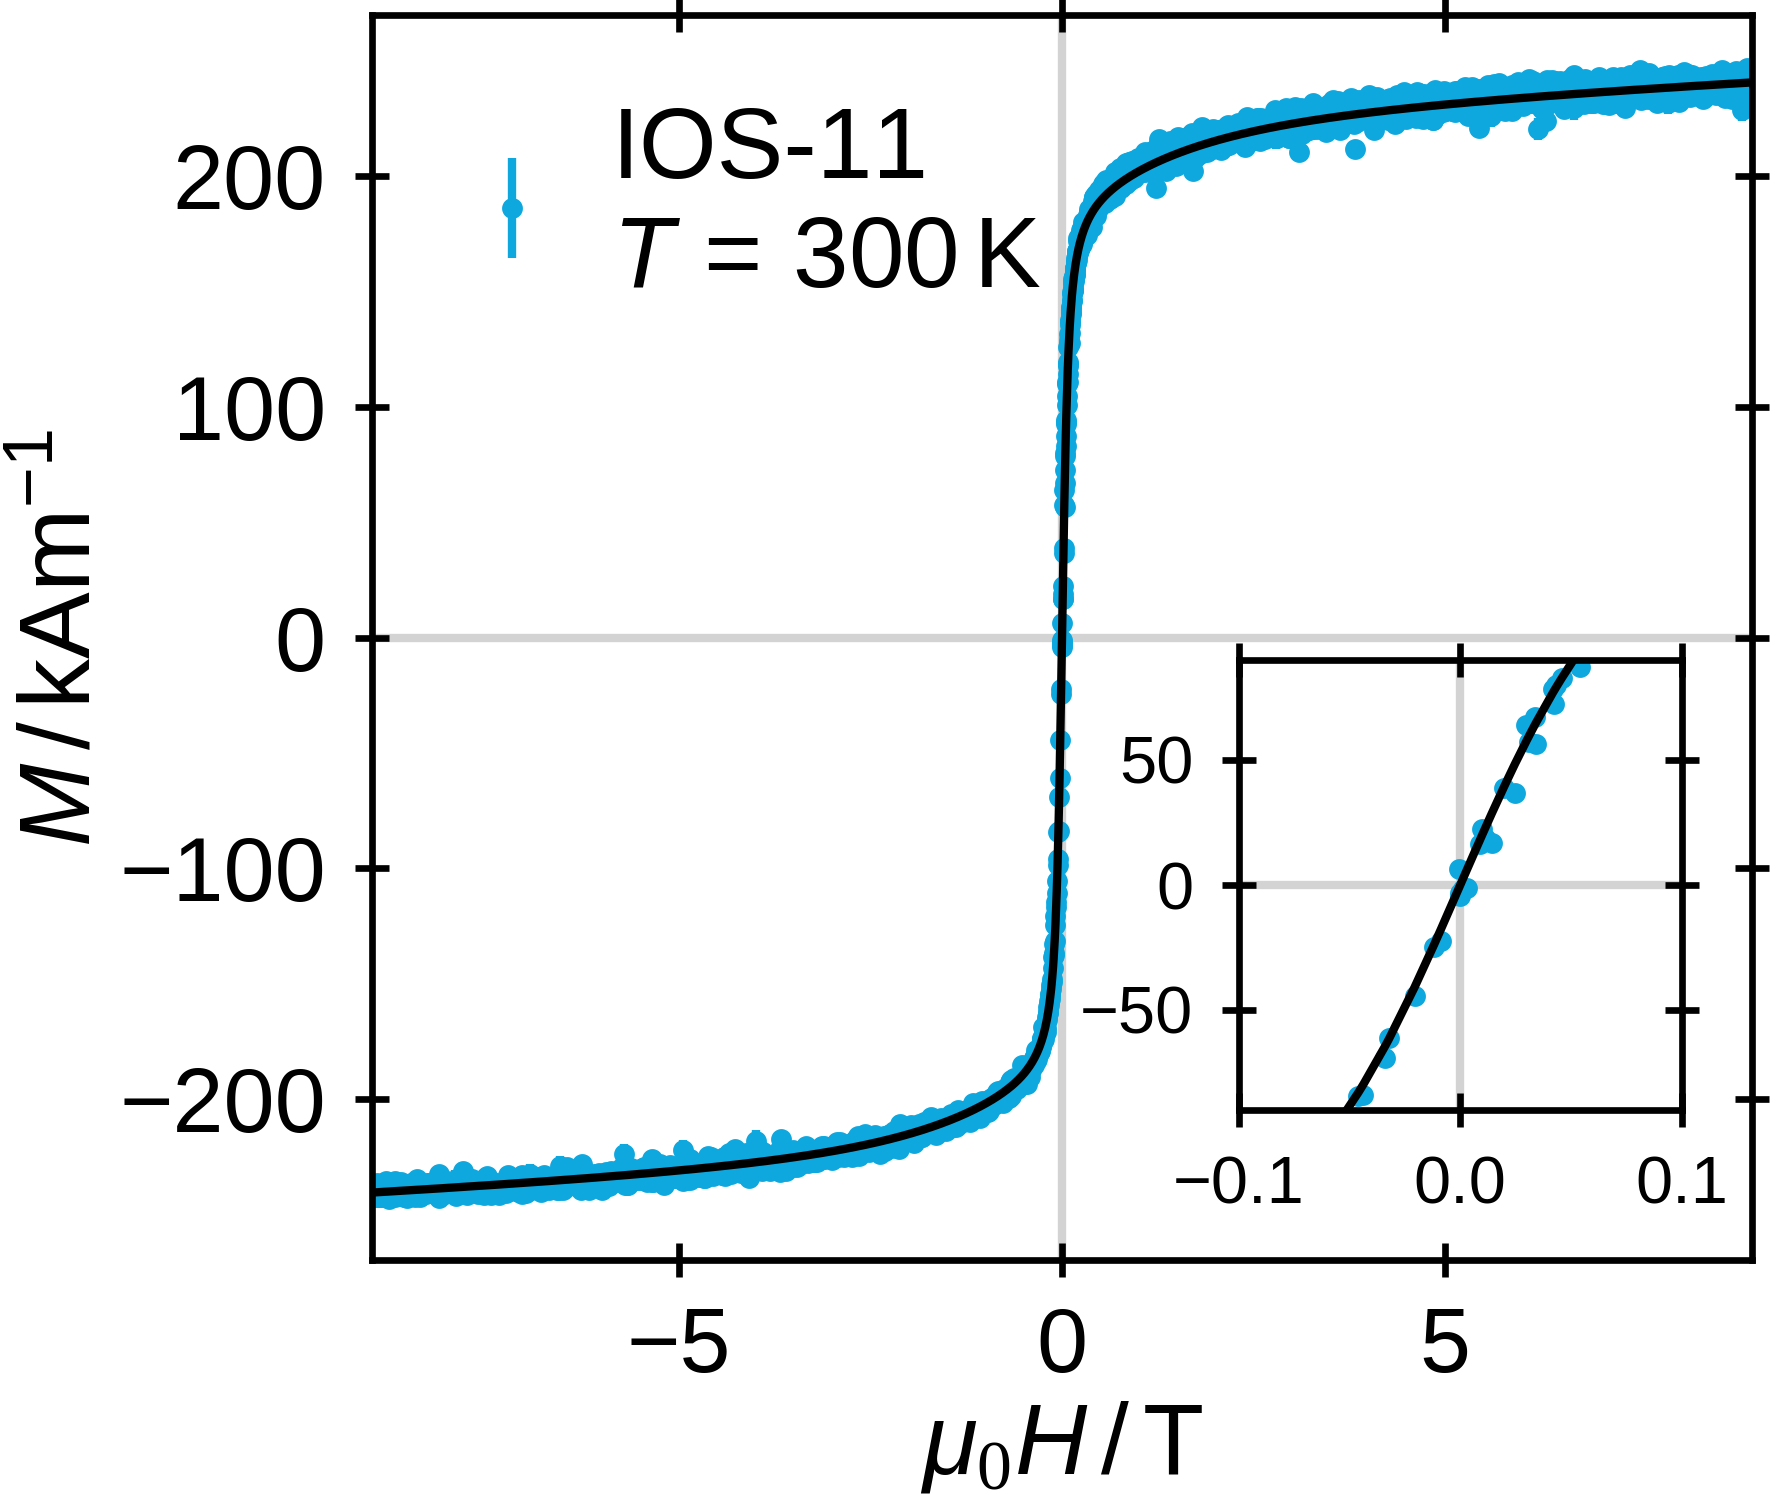
\includegraphics{looselyPackedNP_VSM_IOS-11}
    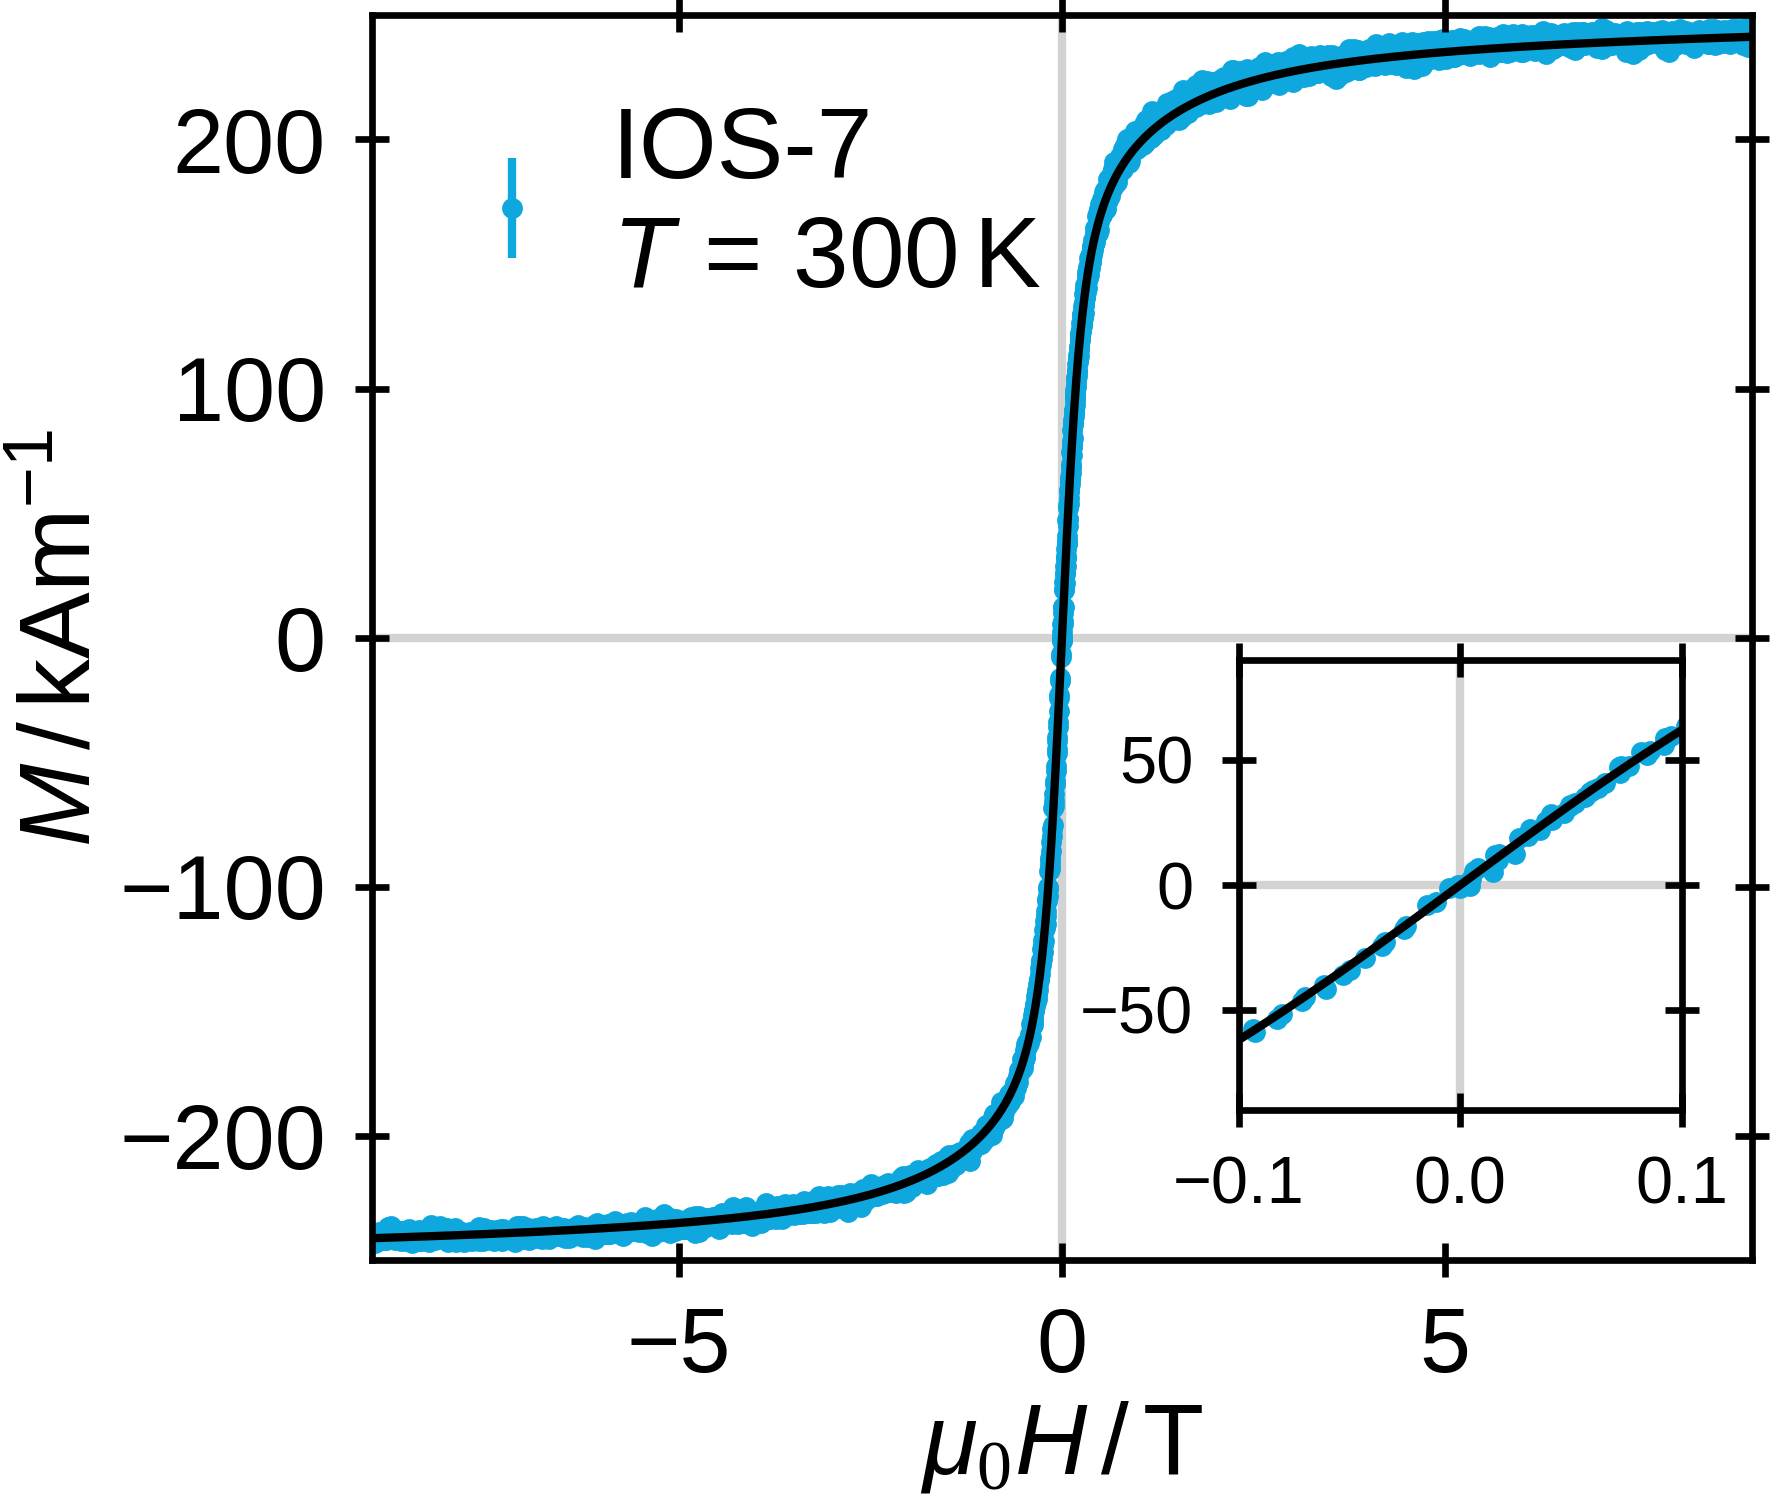
\includegraphics{looselyPackedNP_VSM_IOS-7}
    \caption{\label{fig:looselyPackedNP:nanoparticle:vsm}Room temperature vibrating sample magnetometry for IOS-11 (left) and IOS-7 (right). In black a Langevin behaviour with excess susceptibility is fit and the parameters are given in \reftab{tab:looselyPackedNP:nanoparticle:vsm}}
  \end{figure}

  Vibrating sample magnetometry is used to probe the macroscopic magnetization of IOS-11 and IOS-7.
  The measured magnetization of the dispersion at $300 \unit{K}$ is shown in \reffig{fig:looselyPackedNP:nanoparticle:vsm}.
  In both cases a superparamagnetic phase is observed, which is parameterized by fitting the data with a linear combination of two Langevin curves with an additional linear term for the excess susceptibility.
  The parameters for the fitted magnetization curves are given in \reftab{tab:looselyPackedNP:nanoparticle:vsm}.

  \begin{table}[!htbp]
    \centering
    \caption{\label{tab:looselyPackedNP:nanoparticle:vsm} Parameters determined from field- and temperature-dependent magnetization measurements. From the Langevin behaviour fit, $\mu_i$ is the single-particle magnetic moment and $M_{s,\,i}$ the spontaneous magnetization, where $i\eq 1,\,2$ for refining a linear combination of two modes. $\chi$ is additionally an excess susceptibility. In the low temperature measurements, $H_C$ describes the coercive field, $\Delta H$ the shift observed between ZFC, and FC measured hysteresis curves and $T_B$ is the blocking temperature determined from temperature-dependent VSM.}
    \begin{tabular}{ l | l | l }
      \rule{0pt}{2ex} \textbf{Field-dep. VSM @ 300 K} & IOS-11 & IOS-7 \\
      \hline
      \rule{0pt}{2ex} $\mu_1 \, / \, \mu_B$                     & $13931(72)$    & $4140(13)$\\
      \rule{0pt}{2ex} $\mu_2 \, / \, \mu_B$                     & $485(17) $     & $530(15)$ \\
      \rule{0pt}{2ex} $M_{s,\,1} \, /  \unit{kA\,m^{-1}}$       & $208(1)$       & $216(1)$  \\
      \rule{0pt}{2ex} $M_{s,\,2} \, /  \unit{kA\,m^{-1}}$       & $41(1)$        & $40(1)$   \\
      \rule{0pt}{2ex} $\mu_0 \chi \, / \, 10^{-6}$              & $1991(102)$    & $466(59)$ \\
      \hline
      \hline
      \rule{0pt}{2ex} \textbf{Field-dep. VSM @ 30 K} &  & \\
      \rule{0pt}{2ex} $\mu_0 H_C \, / \unit{mT}$                & $15(2)$        & $10(1)$ \\
      \rule{0pt}{2ex} $\mu_0 \Delta H \, / \unit{mT}$           & $-16(1)$       & $-9(1)$ \\
      \hline
      \hline
      \rule{0pt}{2ex} \textbf{Temp.-dep. VSM @ 10 mT} &  & \\
      \rule{0pt}{2ex} $T_B \, / \unit{K}$                       & $95.5(5)$      & $46.5(5)$ \\
      \rule{0pt}{2ex} $K \, / \unit{10^{5} J m^{-3}}$           & $5.0(1)$       & $8.6(1)$  \\
    \end{tabular}
  \end{table}

  For the nanospheres IOS-11, a magnetic moment of $13931(72) \mu_B$ in the primary mode is observed, which corresponds with the particle size determined from SAS to a spontaneous magnetization of $208(1) \unit{kA\,m^{-1}}$.
  The second mode with the smaller magnetic moment of $485(17) \mu_B$ is necessary to properly describe the data in the intermediate field range above $1 \unit{T}$.
  Using the same rescaling factor, as for the first mode, the second mode has a spontaneous magnetization of $41(1) \unit{kA\,m^{-1}}$.
  To properly describe the non-vanishing slope at high fields, a linear term with positive slope $\mu_0 \chi \eq 1991(102) \cdot 10^{-6}$ is fit.

  The spontaneous magnetization of the nanospheres can be compared to SANSPOL, where an average particle magnetization of $220(14) \unit{kA \, m^{-1}}$ has been observed, and is therefore in excellent agreement.
  The positive paramagnetic slope is smaller than the literature value that would be expected from w\"ustite ($7229 \cdot 10^{-6}$ \cite{Lide_2004_Handb}).
  This indicates also that the w\"ustite phase is not present in the sample but the observed magnetization is a result of the inverse spinell phase in combination with the anti-phase boundaries in the particle volume, as well as possible surface disorder that possibly be the origin of the paramagnetic contribution.
  \\

  The same analysis performed for IOS-7 show by the room temperature VSM a primary mode of $4140(13) \unit{mu_B}$, which corresponds to a magnetization of $216(1) \unit{kA m^{-1}}$.
  In comparison to the SANSPOL result of $151(10) \unit{kA m^{-1}}$, the VSM value is larger, which indicates a systematic error that might have been made by neglecting either the bimodal distribution that was observed in TEM (\refsec{sec:looselyPackedNS:nanoparticle:tem}) or in the surfactant shell thickness, which is not well resolved from the observation of only a single form factor minima.
  The moment of $530(15) \mu_B$ and the spontaneous magnetization of the second mode ($40(1) \unit{kA\,m^{-1}}$) is of similar order as for IOS-11 hinting to a possible similar nature of origin.
  The positive paramagnetic slope of $466(59) \cdot 10^{-6}$ is significantly lower than for IOS-11 and closer to a value of zero.
  This would connect to the observation of a smaller magnetically dead surface layer in SANSPOL and therefore for a smaller shell of disordered spins that give a paramagnetic contribution.

  \begin{figure}[tb]
    \centering
    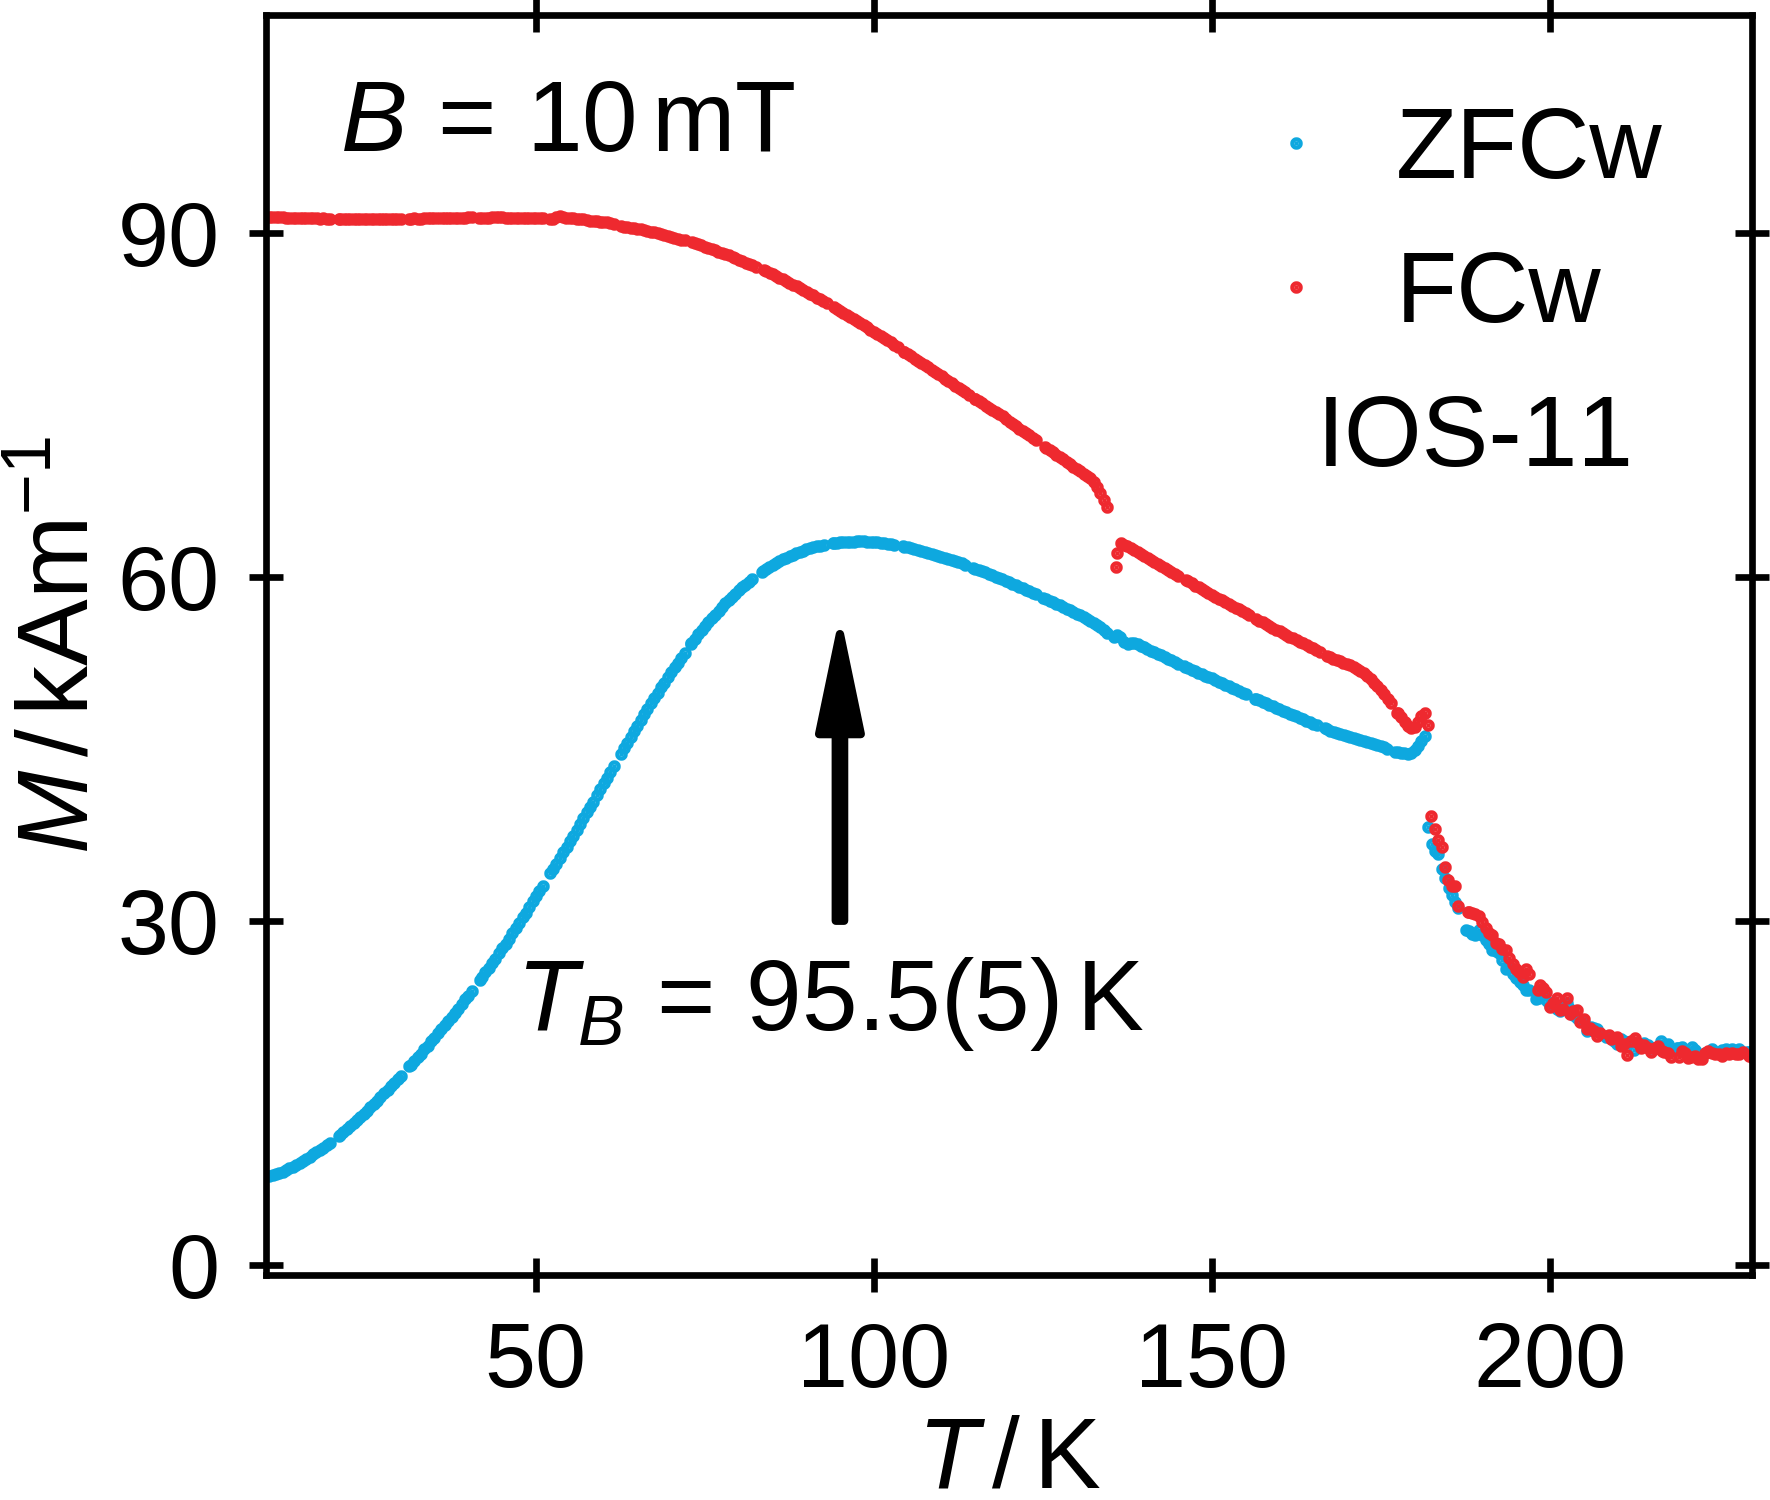
\includegraphics{looselyPackedNP_VSM_ZFC_FC_IOS-11}
    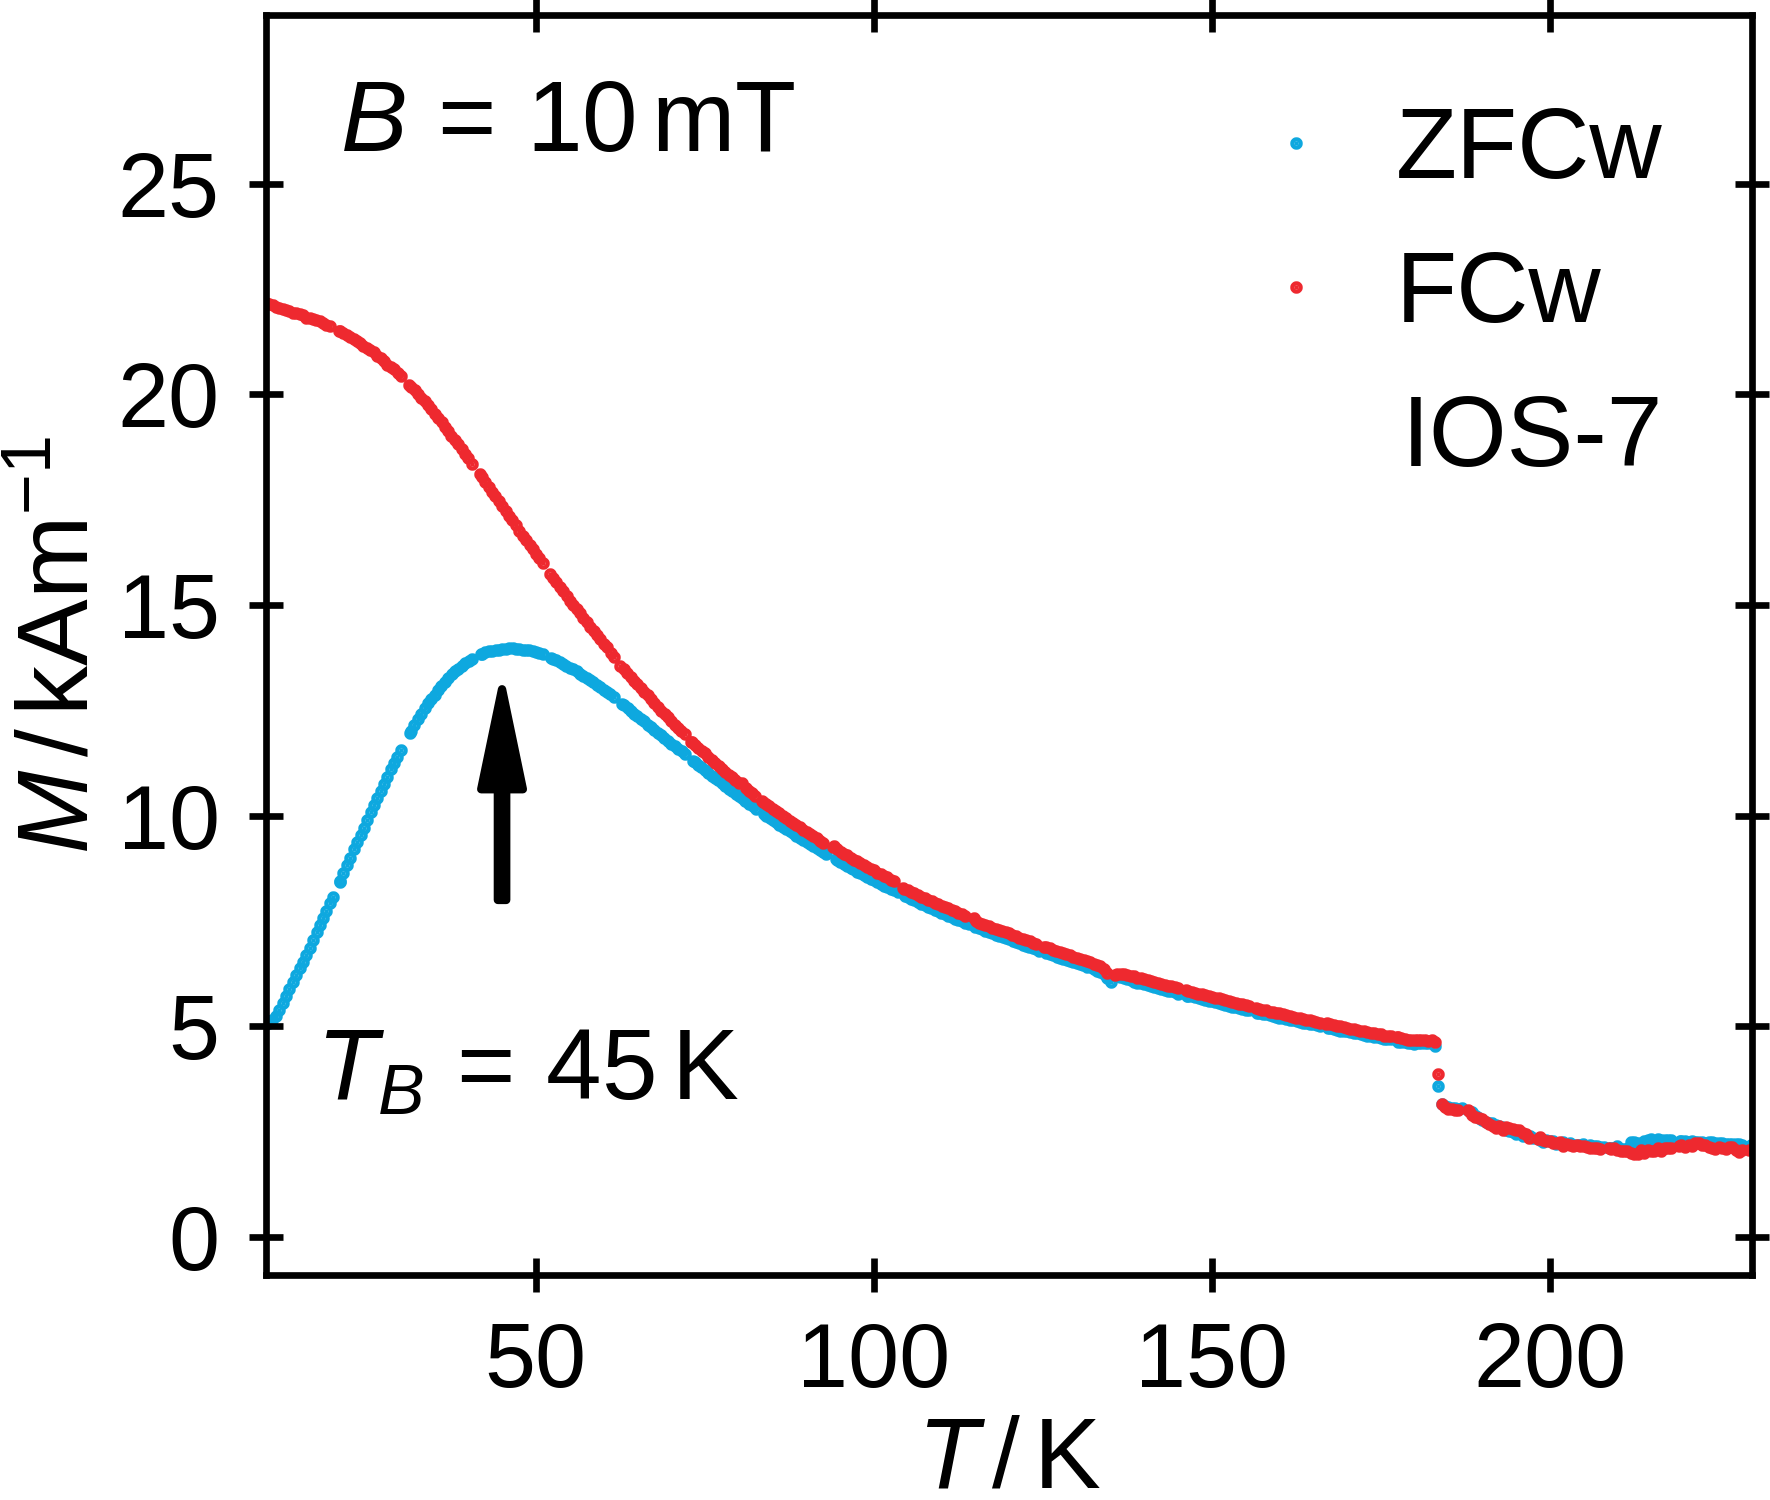
\includegraphics{looselyPackedNP_VSM_ZFC_FC_IOS-7}
    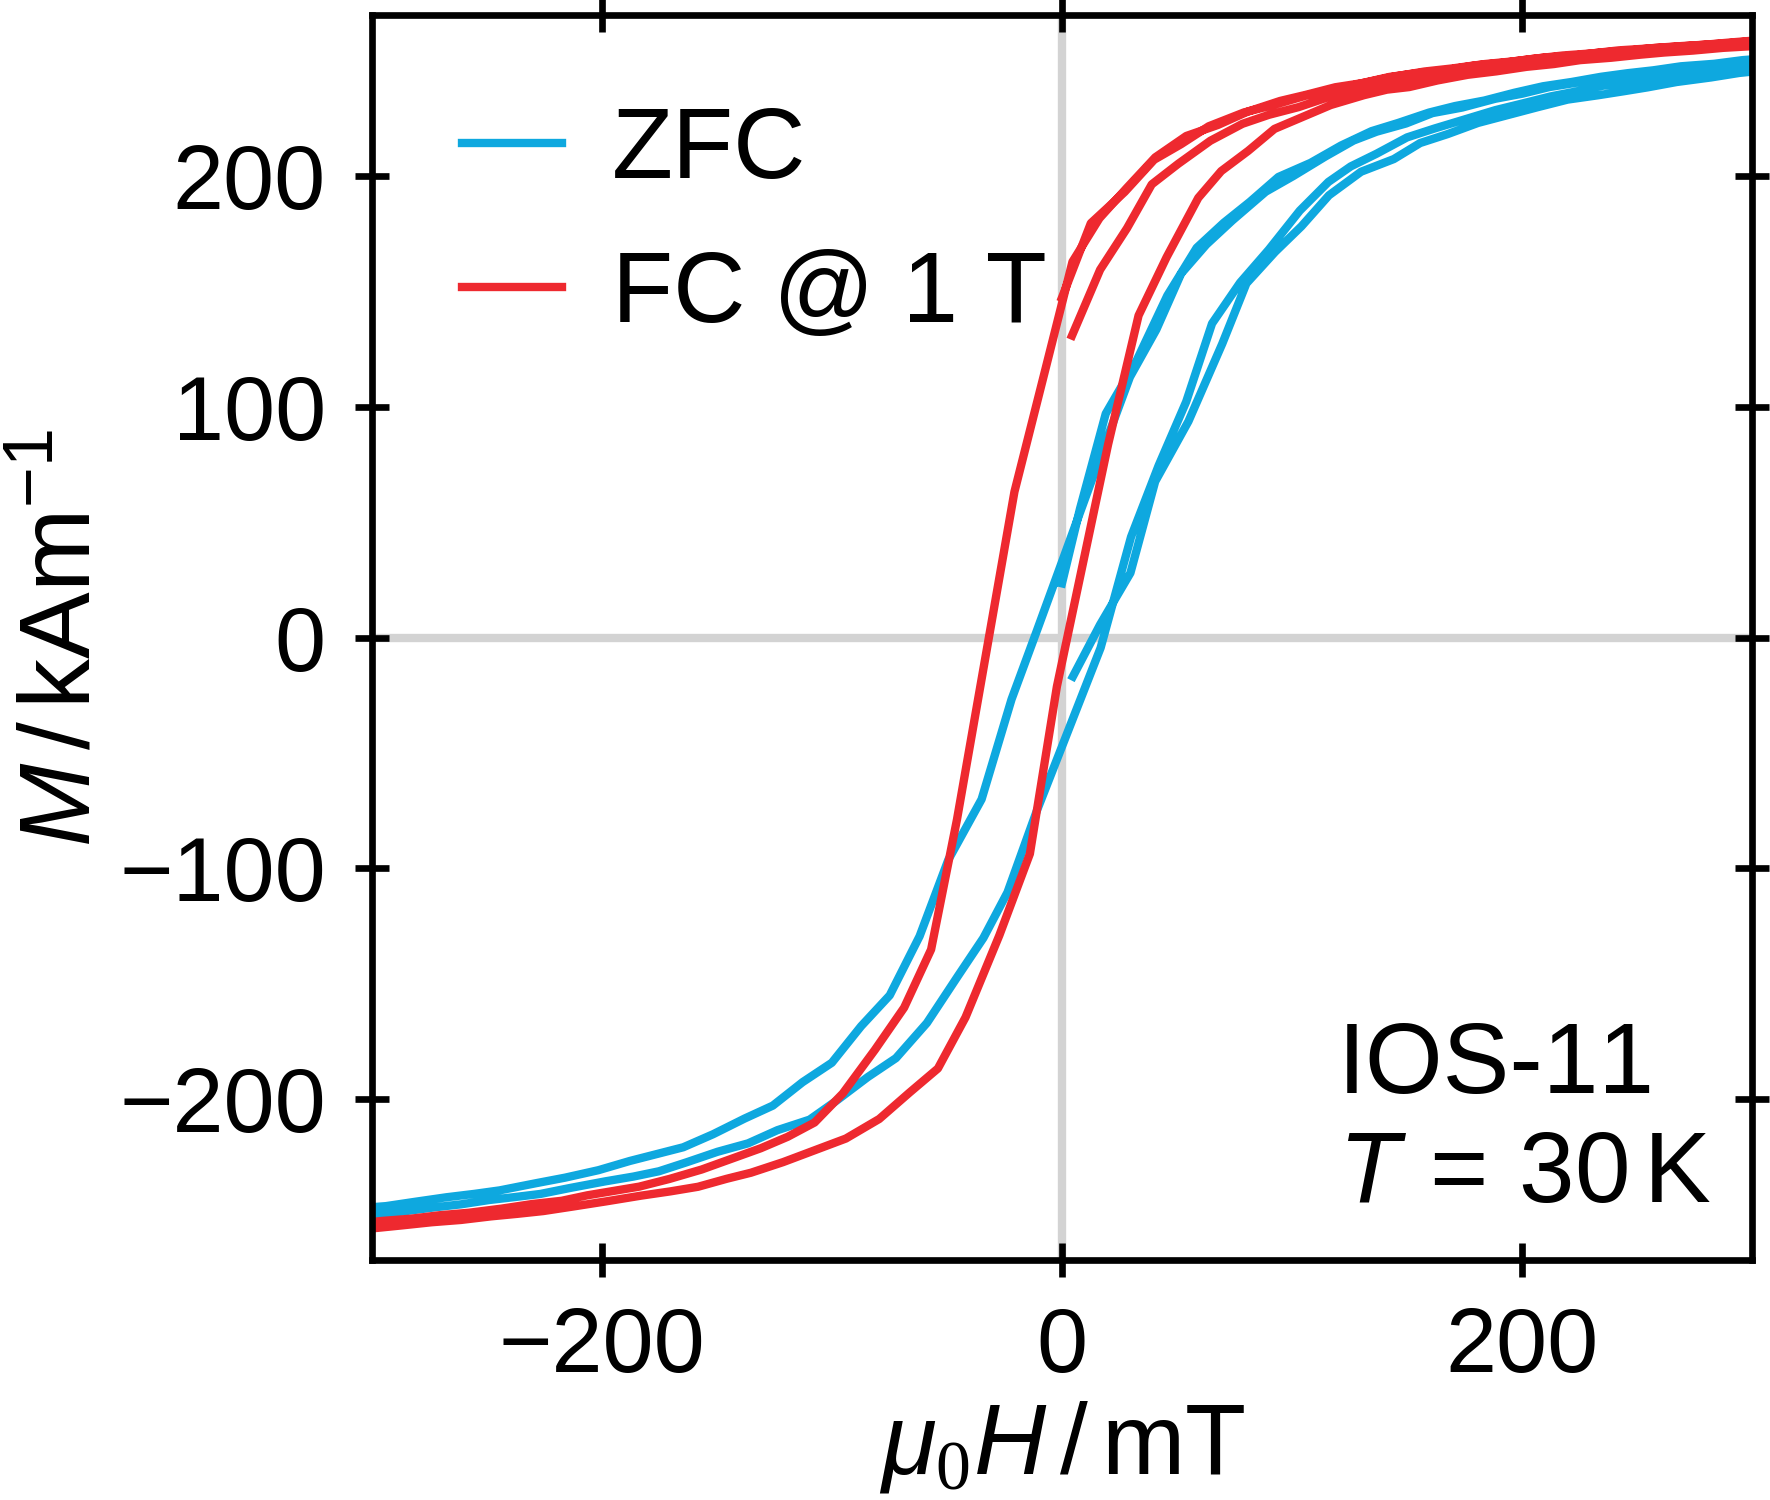
\includegraphics{looselyPackedNP_VSM_30K_IOS-11}
    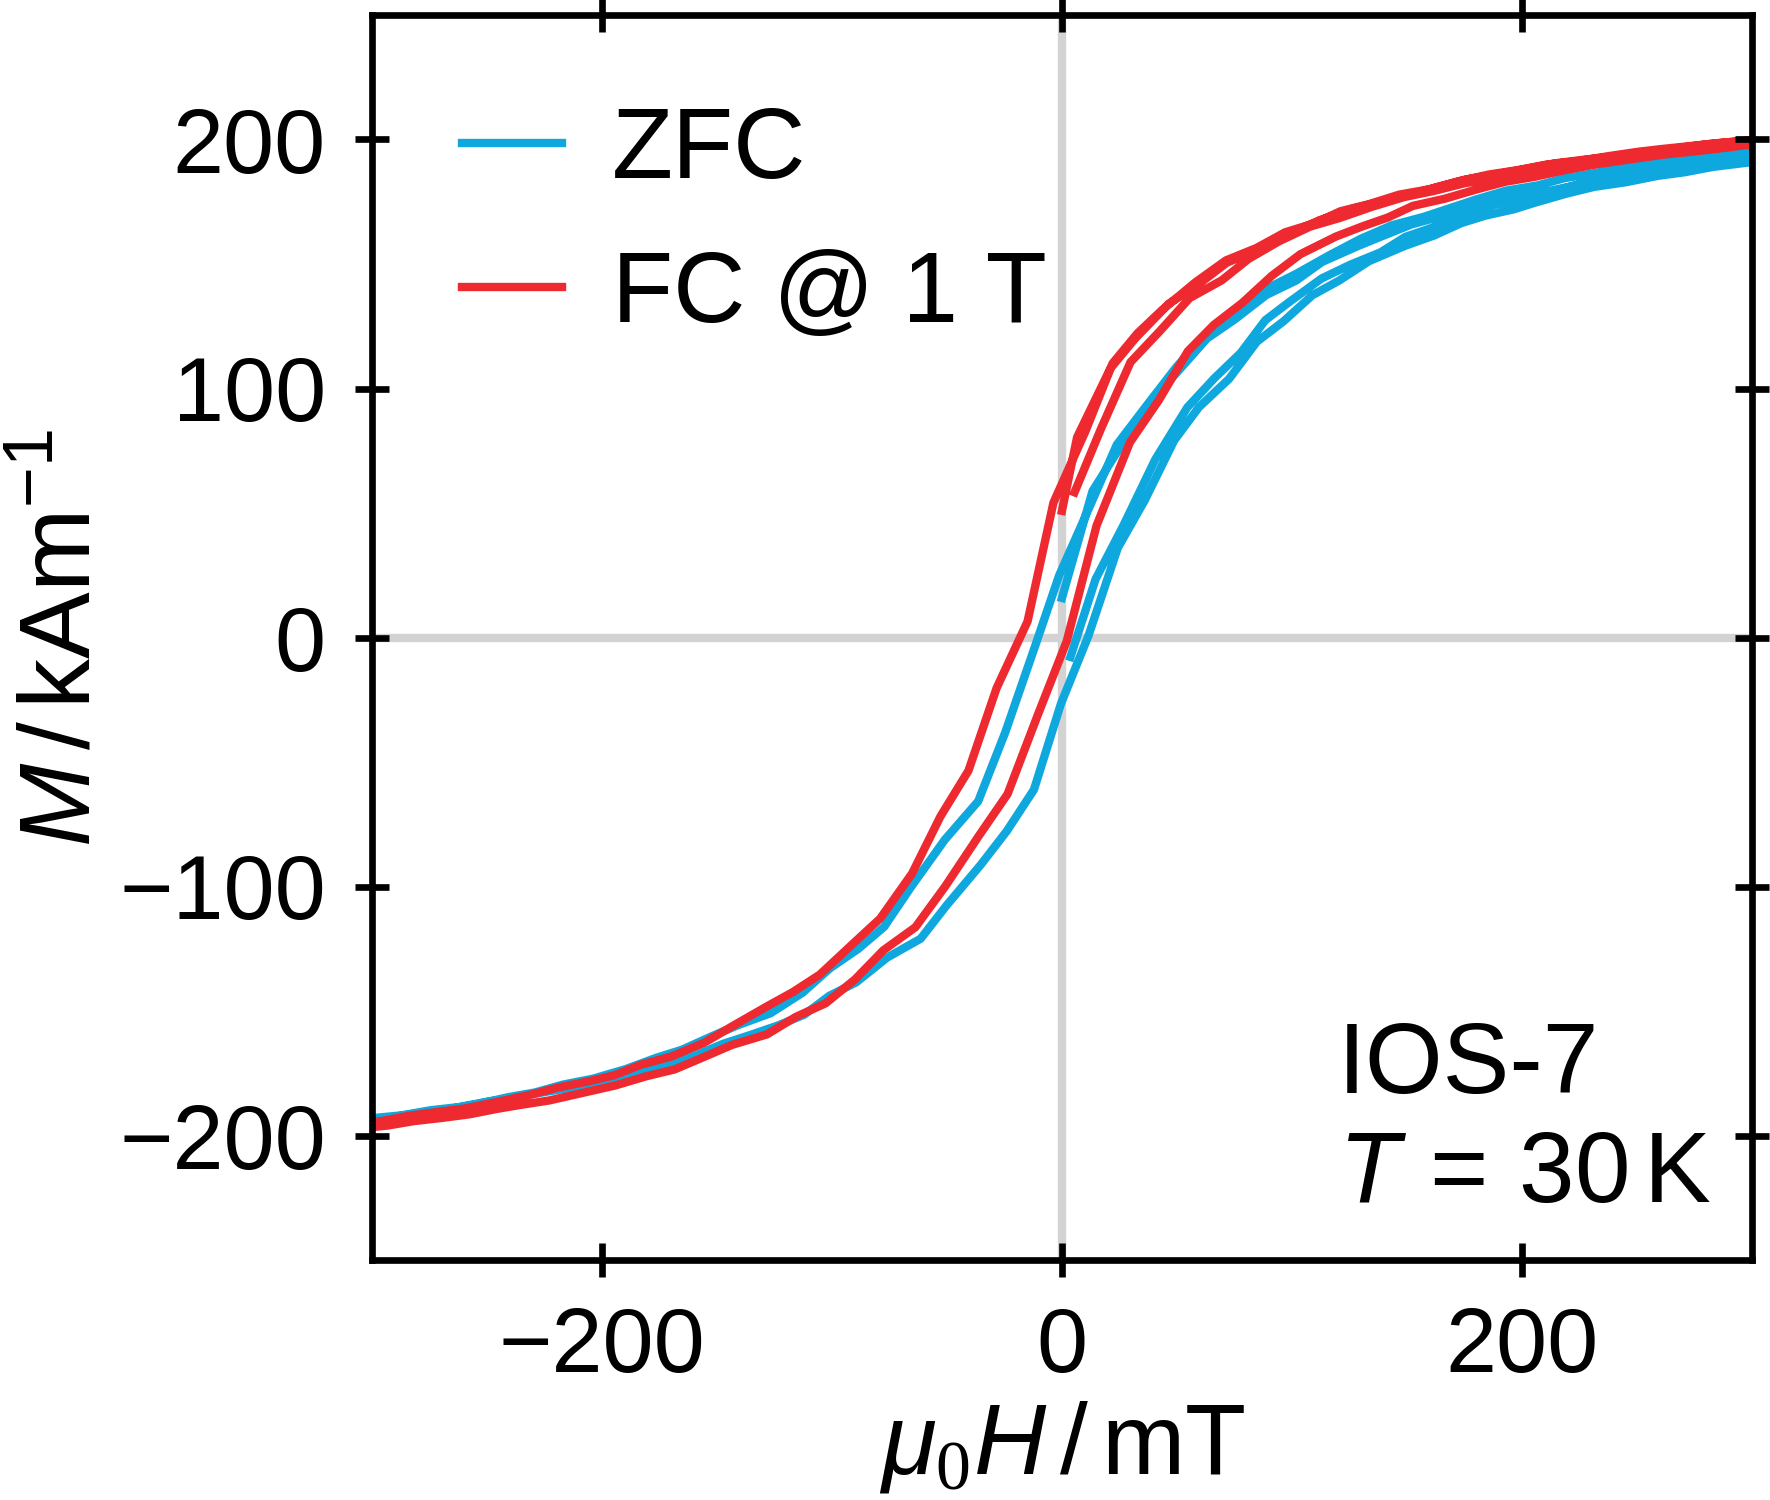
\includegraphics{looselyPackedNP_VSM_30K_IOS-7}
    \caption{\label{fig:looselyPackedNP:nanoparticle:vsm10}Temperature-dependent magnetization measured at $10 \unit{mT}$ after cooling in zero-field and at a field of $10 \unit{mT}$ (upper) for IOS-11 (left) and IOS-7 (right). Additionally shown are low-temperature hysteresis measurements of both samples at $30 \unit{K}$ (upper).}
  \end{figure}
  The temperature dependent magnetization in \reffig{fig:looselyPackedNP:nanoparticle:vsm10} yields the blocking temperature of IOS-11 to be at $95.5(5) \unit{K}$ and for IOS-7 at $46.5(5) \unit{K}$, which is determined by the maximum of the zero-field cooled magnetization measurement.
  The significantly smaller values observed for IOS-7 is connected to the smaller particle size of the nanospheres.
  Using \refeq{eq:theoreticalBackground:superparamagnetism:blockingTemp} and the particle volume determined from SAS, the magnitude of the effective magnetocrystalline anisotropy constant $K$ is estimated with $\log(\tau_m / \tau_0) \approx 25$ to $5.0(1) \cdot \unit{10^{5} J m^{-3}}$ and $8.6(1)\cdot \unit{10^{5} J m^{-3}}$ for IOS-11 and IOS-7 respectively.
  In comparison to this, the literature value for bulk magnetite is found to be slightly larger as $K_1 \eq -13.5 \cdot  \unit{10^{5} J m^{-3}}$ \cite{Goya_2003_Stati} but in a similar order of magnitude.
  Deviations are possible, as the previous nanoparticle characterization has already shown that the nanoparticles are not equivalent to perfectly crystalline magnetite due to the presence of anti-phase boundaries and possibly surface disorder.

  In the temperature-dependent magnetization of IOS-11, an additional jump is observed around $135 \unit{K}$, this jump is close to the Verwey transition in magnetite, which is expected to be around $125 \unit{K}$ \cite{Walz_2002_Theve} and the isotropic point of magnetite at $130 \unit{K}$, where the magnetocrystalline anisotropy changes it's sign \cite{Muxworthy_1999_Lowte}.
  Below the Verwey temperature, magnetite is known to change from a cubic inverse spinel structure to a monoclinic structure.
  This transition is not clearly visible in the temperature-dependent magnetization measurement of IOS-7, but a small dip also appears here at $135 \unit{K}$.

  At low temperatures of $30 \unit{K}$, the magnetization of IOS-11 and IOS-7 in \reffig{fig:looselyPackedNP:nanoparticle:vsm10} show a hysteretic behaviour, which is strongly dependent on whether the sample is cooled in zero field or cooled while a strong magnetic field.
  From the zero-field cooled curve, IOS-11 has a coercive field of $15(2) \unit{mT}$ and IOS-7 a field of $10(1) \unit{mT}$, which is shifted by $16(1) \unit{mT}$ and $9(1) \unit{mT}$ respectively towards negative field upon application of $1 \unit{T}$ during the cooling procedure from $300 \unit{K}$ to $30 \unit{K}$.
  The coercive fields are slightly lower than the $30 \unit{mT}$ resulting from crystal anisotropy found in literature for magnetite \cite{Cornell_2003_Their}.
  The smaller magnitudes is a result for one from the already to be smaller determined magnetocrystalline anisotropy and from measuring at a slightly elevated temperature of $30 \unit{K}$ and not closer to $0 \unit{K}$, which is done for a better direct comparison to results later discussed in the framework of polarized neutron reflectometry.
  As the measurement temperature approaches the blocking temperature, the superparamagnetic phase becomes noticeable by the vanishing of the hysteresis and the coercive field going to zero.
  The shift in magnetization is also observed in literature for non-interacting oleate based iron oxide nanoparticles that does not vanish with complete oxidation of the nanoparticles \cite{Wetterskog_2013_Anoma}.
  It's an effect from the regions in the nanoparticle volume that are separated by an anti-phase boundary.
  \\

  Concludingly, the VSM analysis of the nanoparticle dispersions confirms for one by the room temperature measurements the SANSPOL results by a complimentary method and for the other provides additional information on the temperature dependent magnetization behaviour of the nanospheres.
  The blocking temperatures reveal that temperatures significantly below $50 \unit{K}$ should be chosen for the discussion of the nanoparticle magnetization to avoid thermal averaging from the superparamagnetic phase.
  Furthermore a significant difference is observed between zero-field and field cooled nanoparticles, which manifest in an exchange bias shift of the hysteresis.
\end{document}